 \documentclass[a4paper,10pt]{article}
\input{/Users/WannaGetHigh/workspace/latex/macros.tex}

\title{TI TP5 : Transformations ponctuelles sous ImageJ}
\author{Fran�ois \bsc{Lepan}}

\begin{document}
\maketitle

\section{Loi de correction affine $g(x,y) = a +b.I(x,y)$ � appliquer sur la LUT d'affichage
de telle sorte que la dynamique des niveaux affich�s soit comprise entre 0 et 255}

Voici le code la macro correspondante:
\begin{Verbatim}[commandchars=\\\{\}]
\codeBlue{// recherche du min et du max}

min = 255;
max = 0;

for (j=0; j<H; j++) 
\{
   	for (i=0; i<W; i++) 
	\{
		p = getPixel(i,j);
		if ( min > p)
		\{
			min =p;
		\}

	       if (max < p)
		\{
			max = p;
		\}
	\}
\}

print ("min =", min);
print ("max =", max);

\codeBlue{// d�claration des LUTs}

    reds = newArray(256); 
    greens = newArray(256); 
    blues = newArray(256);

\codeBlue{// R�cup�ration des LUTS}
    getLut(reds, greens, blues);

\codeBlue{// On applique la loi de correction affine}
\codeBlue{// de telle sorte que la dynamique des niveaux affich�s soit comprise entre 0 et 255.}

\codeBlue{// Tout d'abord on met les valeurs inf�rieur � min � la valeur minimale 0}
for (i=0; i<min; i++) \{
	reds[i] = 0;
	greens[i] = 0;
	blues[i] = 0;
\}

\codeBlue{// On applique la loi de correction affine sur}
\codeBlue{// les valeurs comprise entre min et max}
for (i=min; i<max; i++) \{
	reds[i] = ((i-min)*255/(max-min));
	greens[i] = ((i-min)*255/(max-min));
 	blues[i] = ((i-min)*255/(max-min));
\}

\codeBlue{// Et enfin on met les valeurs sup�rieur ou �gale � max � la valeur maximale 255}
for (i=max; i<reds.length; i++) \{
	reds[i] = 255;
	greens[i] = 255;
	blues[i] = 255;
\}
\end{Verbatim}

L'�xecution de ce code nous fournis la Fig.~\ref{fig:lena_correction_affine_Q1} sur laquelle on peut voir l'image de Lena diff�rente de celle de base (\emph{cf: Fig.}\ref{fig:lena-ndg}) 

\begin{figure}[H]
	\begin{center}
		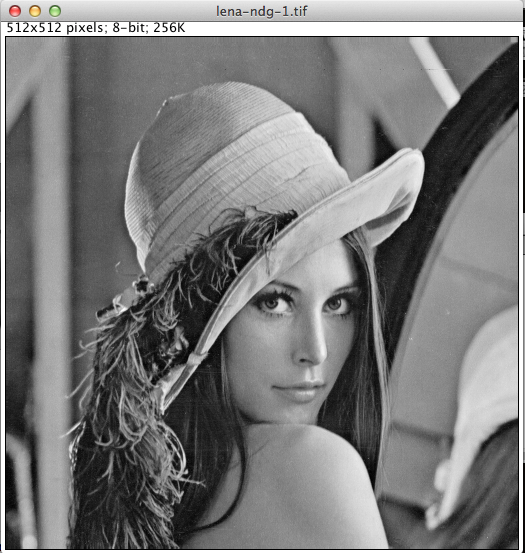
\includegraphics[width=8cm]{lena_correction_affine_Q1.png}
	\end{center}
	\caption{Image de Lena modifi�e gr�ce � la loi de correction affine $g(x,y) = a +b.I(x,y)$}
	\label{fig:lena_correction_affine_Q1}
\end{figure}

\begin{figure}[H]
	\begin{center}
		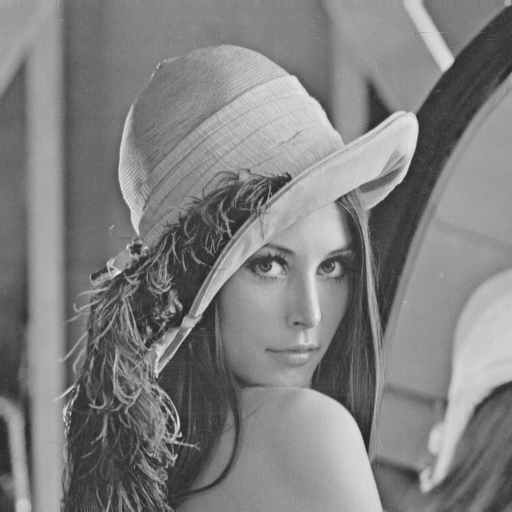
\includegraphics[width=8cm]{lena-ndg.png}
	\end{center}
	\caption{Image de Lena initiale}
	\label{fig:lena-ndg}
\end{figure}

\section{La modification de la LUT agit-elle sur les niveaux de gris des pixels ?}

Non le niveau de gris des pixels reste inchang� (\emph{cf: Fig.}\ref{fig:histo_lena_modif_fonc_aff}). Et c'est normal car la modification de la LUT ne modifie que l'aspect visuel et non la valeur de chaque pixel (\emph{cf: Fig.}\ref{fig:ti_LUT_explanation}).

\begin{figure}[H]
	\begin{center}
		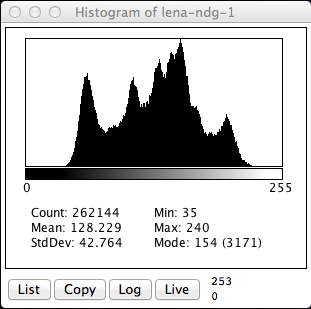
\includegraphics[width=8cm]{histo_lena_modif_fonc_aff.png}
	\end{center}
	\caption{Histogramme de l'image Lena modifi�}
	\label{fig:histo_lena_modif_fonc_aff}
\end{figure}

\begin{figure}[H]
	\begin{center}
		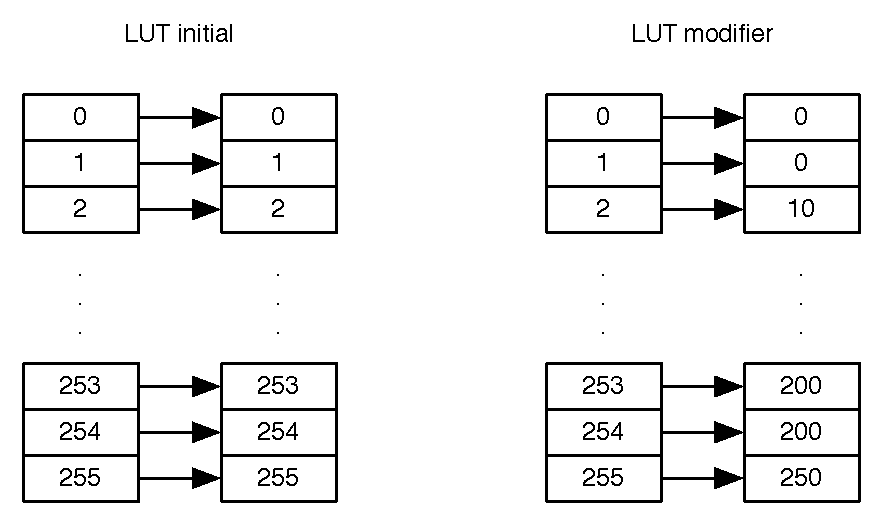
\includegraphics[width=10cm]{graphics/ti_LUT_explanation.pdf}
	\end{center}
	\caption{Explication: LUT initial -> LUT modifi�e}
	\label{fig:ti_LUT_explanation}
\end{figure}

\newpage

\section{Modification des niveaux de gris des pixels pour que la dynamique des niveaux de gris soit comprise entre 0 et 255}

Voici le code la macro correspondante:
\begin{Verbatim}[commandchars=\\\{\}]

for (j=0; j<H; j++) 
\{
	for (i=0; i<W; i++) 
	\{
		p = getPixel(i,j);
		setPixel(i,j,reds[p]);
	\}
\}
\end{Verbatim}

Apr�s avoir �talonn� les valeurs pour la LUT (voir code question 1), il suffit de parcourir l'image et d'appliqu� aux pixels la valeur trouv�. On obtient la Fig.~\ref{fig:histogramme_valeurs_modif} sur laquelle on observe un l'histogramme des niveau de gris. On voit bien que les valeurs sont plus �tal�es que sur l'histogramme de la Fig. \ref{fig:histo_lena_modif_fonc_aff}.

\begin{figure}[H]
	\begin{center}
		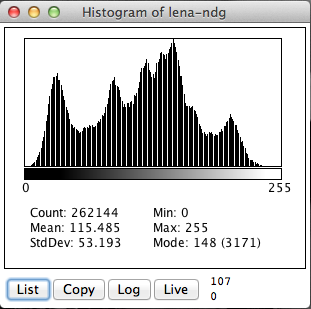
\includegraphics[width=8cm]{histogramme_valeurs_modif.png}
	\end{center}
	\caption{Histogramme de l'image Lena avec les valeurs de niveau de gris directement modifi�}
	\label{fig:histogramme_valeurs_modif}
\end{figure}

\end{document}